\documentclass[border=10pt]{standalone}
\usepackage[T1]{fontenc}
\usepackage{amsmath}
\usepackage{amssymb}
\usepackage{tikz}
\usetikzlibrary{positioning, shapes, arrows.meta, fit, shadows}

\begin{document}

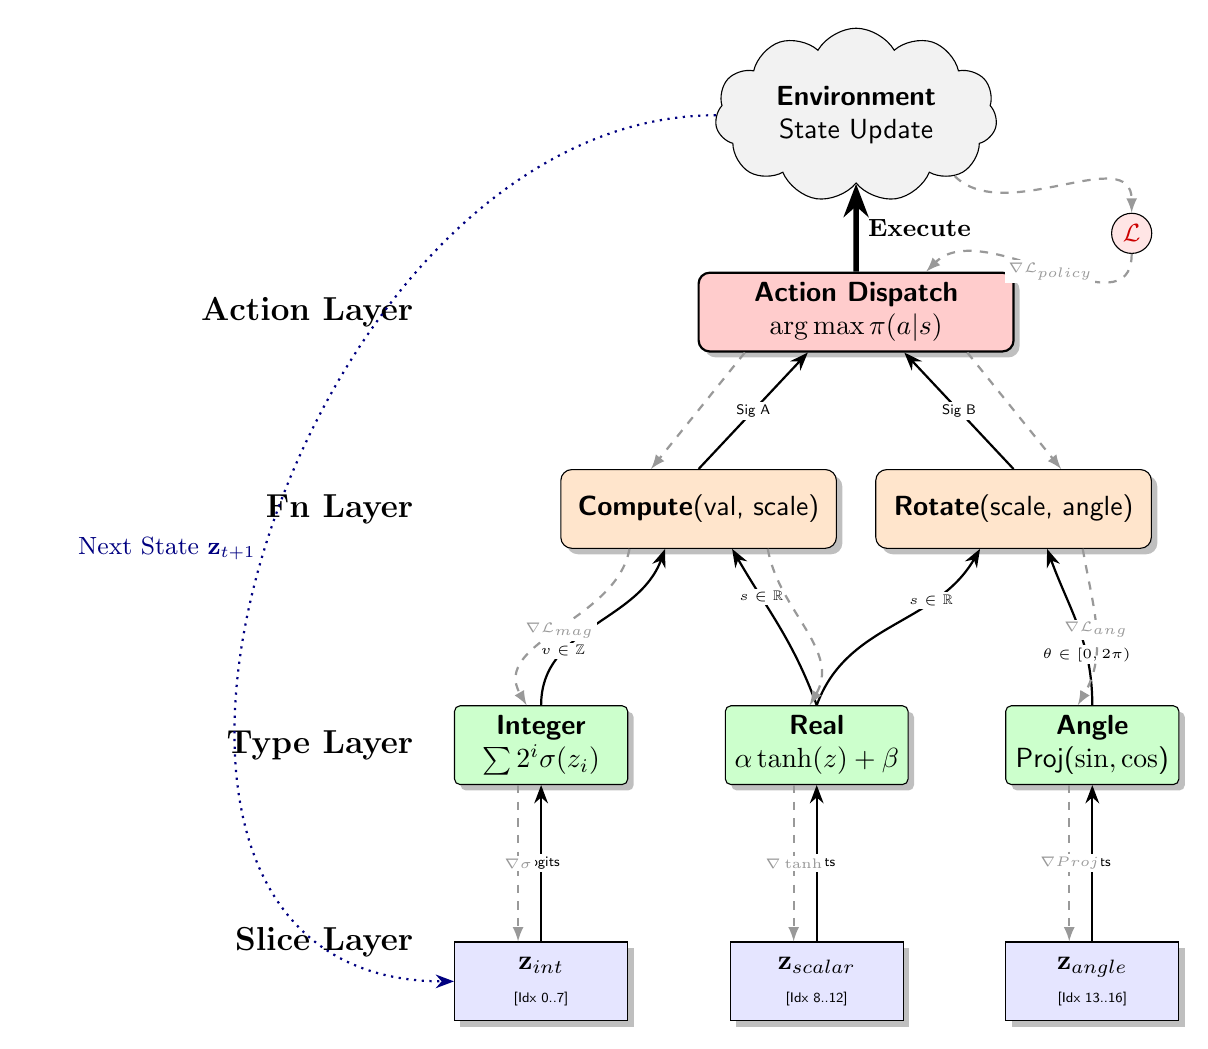
\begin{tikzpicture}[
  font=\sffamily,
  slice/.style={minimum height=1cm, minimum width=2.2cm, draw, fill=blue!10, align=center, drop shadow},
  decode/.style={minimum height=1cm, minimum width=2.2cm, draw, fill=green!20, align=center, rounded corners=2pt, drop shadow},
  fn/.style={minimum height=1cm, draw, fill=orange!20, rounded corners, align=center, drop shadow},
  action/.style={minimum height=1cm, minimum width=4cm, draw, fill=red!20, rounded corners, thick, align=center, drop shadow},
  env/.style={cloud, draw, cloud puffs=11, cloud puff arc=120, aspect=2, fill=gray!10, inner sep=0.2cm, align=center},
  loss/.style={circle, draw, fill=red!10, text=red!80!black, font=\bfseries\small, inner sep=2pt},
  arrow/.style={->, >=Stealth, thick, color=black},
  backprop/.style={->, >=latex, dashed, thick, color=gray!80},
  feedback/.style={->, >=Stealth, dotted, thick, color=blue!50!black},
  layerlabel/.style={anchor=east, font=\bfseries\large},
  typelabel/.style={fill=white, inner sep=1pt, font=\tiny\sffamily, text=black},
  gradlabel/.style={fill=white, inner sep=1pt, font=\tiny\bfseries, text=gray!80}
]

% --- 1. SliceLayer ---
\node[layerlabel] at (-1.5, 0.5) {Slice Layer};
\node[slice] (s1) at (0, 0) {$\mathbf{z}_{int}$ \\ \tiny{[Idx 0..7]}};
\node[slice] (s2) at (3.5, 0) {$\mathbf{z}_{scalar}$ \\ \tiny{[Idx 8..12]}};
\node[slice] (s3) at (7, 0) {$\mathbf{z}_{angle}$ \\ \tiny{[Idx 13..16]}};

% --- 2. TypeLayer ---
\node[layerlabel] at (-1.5, 3) {Type Layer};
\node[decode] (t1) at (0, 3) {\textbf{Integer} \\ $\sum 2^i \sigma(z_i)$};
\node[decode] (t2) at (3.5, 3) {\textbf{Real} \\ $\alpha \tanh(z) + \beta$};
\node[decode] (t3) at (7, 3) {\textbf{Angle} \\ Proj($\sin, \cos$)};

\draw[arrow] (s1.north) -- (t1.south) node[midway, typelabel] {Logits};
\draw[arrow] (s2.north) -- (t2.south) node[midway, typelabel] {Logits};
\draw[arrow] (s3.north) -- (t3.south) node[midway, typelabel] {Logits};

% --- 3. FnLayer ---
\node[layerlabel] at (-1.5, 6) {Fn Layer};
\node[fn, minimum width=3.5cm] (f1) at (2, 6) {\textbf{Compute}(val, scale)};
\node[fn, minimum width=3.5cm] (f2) at (6, 6) {\textbf{Rotate}(scale, angle)};

\draw[arrow] (t1.north) to[out=90, in=250] node[pos=0.3, typelabel] {$v \in \mathbb{Z}$} (f1.230);
\draw[arrow] (t2.north) to[out=110, in=300] node[pos=0.7, typelabel] {$s \in \mathbb{R}$} (f1.310);
\draw[arrow] (t2.north) to[out=70, in=240] node[pos=0.7, typelabel] {$s \in \mathbb{R}$} (f2.230);
\draw[arrow] (t3.north) to[out=90, in=290] node[pos=0.3, typelabel] {$\theta \in [0, 2\pi)$} (f2.310);

% --- 4. ActionLayer ---
\node[layerlabel] at (-1.5, 8.5) {Action Layer};
\node[action] (act) at (4, 8.5) {\textbf{Action Dispatch} \\ $\arg\max \pi(a | s)$};

\draw[arrow] (f1.north) -- (act.220) node[midway, typelabel] {Sig A};
\draw[arrow] (f2.north) -- (act.320) node[midway, typelabel] {Sig B};

% --- 5. Environment & Loss ---
\node[env] (environment) at (4, 11) {\textbf{Environment} \\ State Update};
\node[loss] (loss) at (7.5, 9.5) {$\mathcal{L}$};

\draw[arrow, line width=2pt] (act.north) -- (environment.south) node[midway, right, font=\small\bfseries] {Execute};

% --- Backpropagation ---
\draw[backprop] (environment.south east) to[out=-45, in=90] (loss.north);
\draw[backprop] (loss.south) to[out=270, in=45] node[midway, gradlabel] {$\nabla \mathcal{L}_{policy}$} (act.30);
\draw[backprop] (act.200) -- (f1.140);
\draw[backprop] (act.340) -- (f2.40);
\draw[backprop] (f1.210) to[out=260, in=120] node[midway, gradlabel] {$\nabla \mathcal{L}_{mag}$} (t1.110);
\draw[backprop] (f1.330) to[out=280, in=60] (t2.100);
\draw[backprop] (f2.330) to[out=280, in=60] node[midway, gradlabel] {$\nabla \mathcal{L}_{ang}$} (t3.110);
\draw[backprop] (t1.240) -- (s1.120) node[midway, gradlabel] {$\nabla \sigma$};
\draw[backprop] (t2.240) -- (s2.120) node[midway, gradlabel] {$\nabla \tanh$};
\draw[backprop] (t3.240) -- (s3.120) node[midway, gradlabel] {$\nabla Proj$};

% --- Feedback Loop ---
\draw[feedback] (environment.west) to[out=180, in=180, looseness=1.2] node[midway, left, font=\small] {Next State $\mathbf{z}_{t+1}$} (s1.west);

\end{tikzpicture}

\end{document}